\documentclass{standalone}
\usepackage{tikz}
\usetikzlibrary{patterns, positioning}
\usepackage[sfdefault]{ClearSans} %% option 'sfdefault' activates Clear Sans as the default text font
\usepackage[T1]{fontenc}

\begin{document}
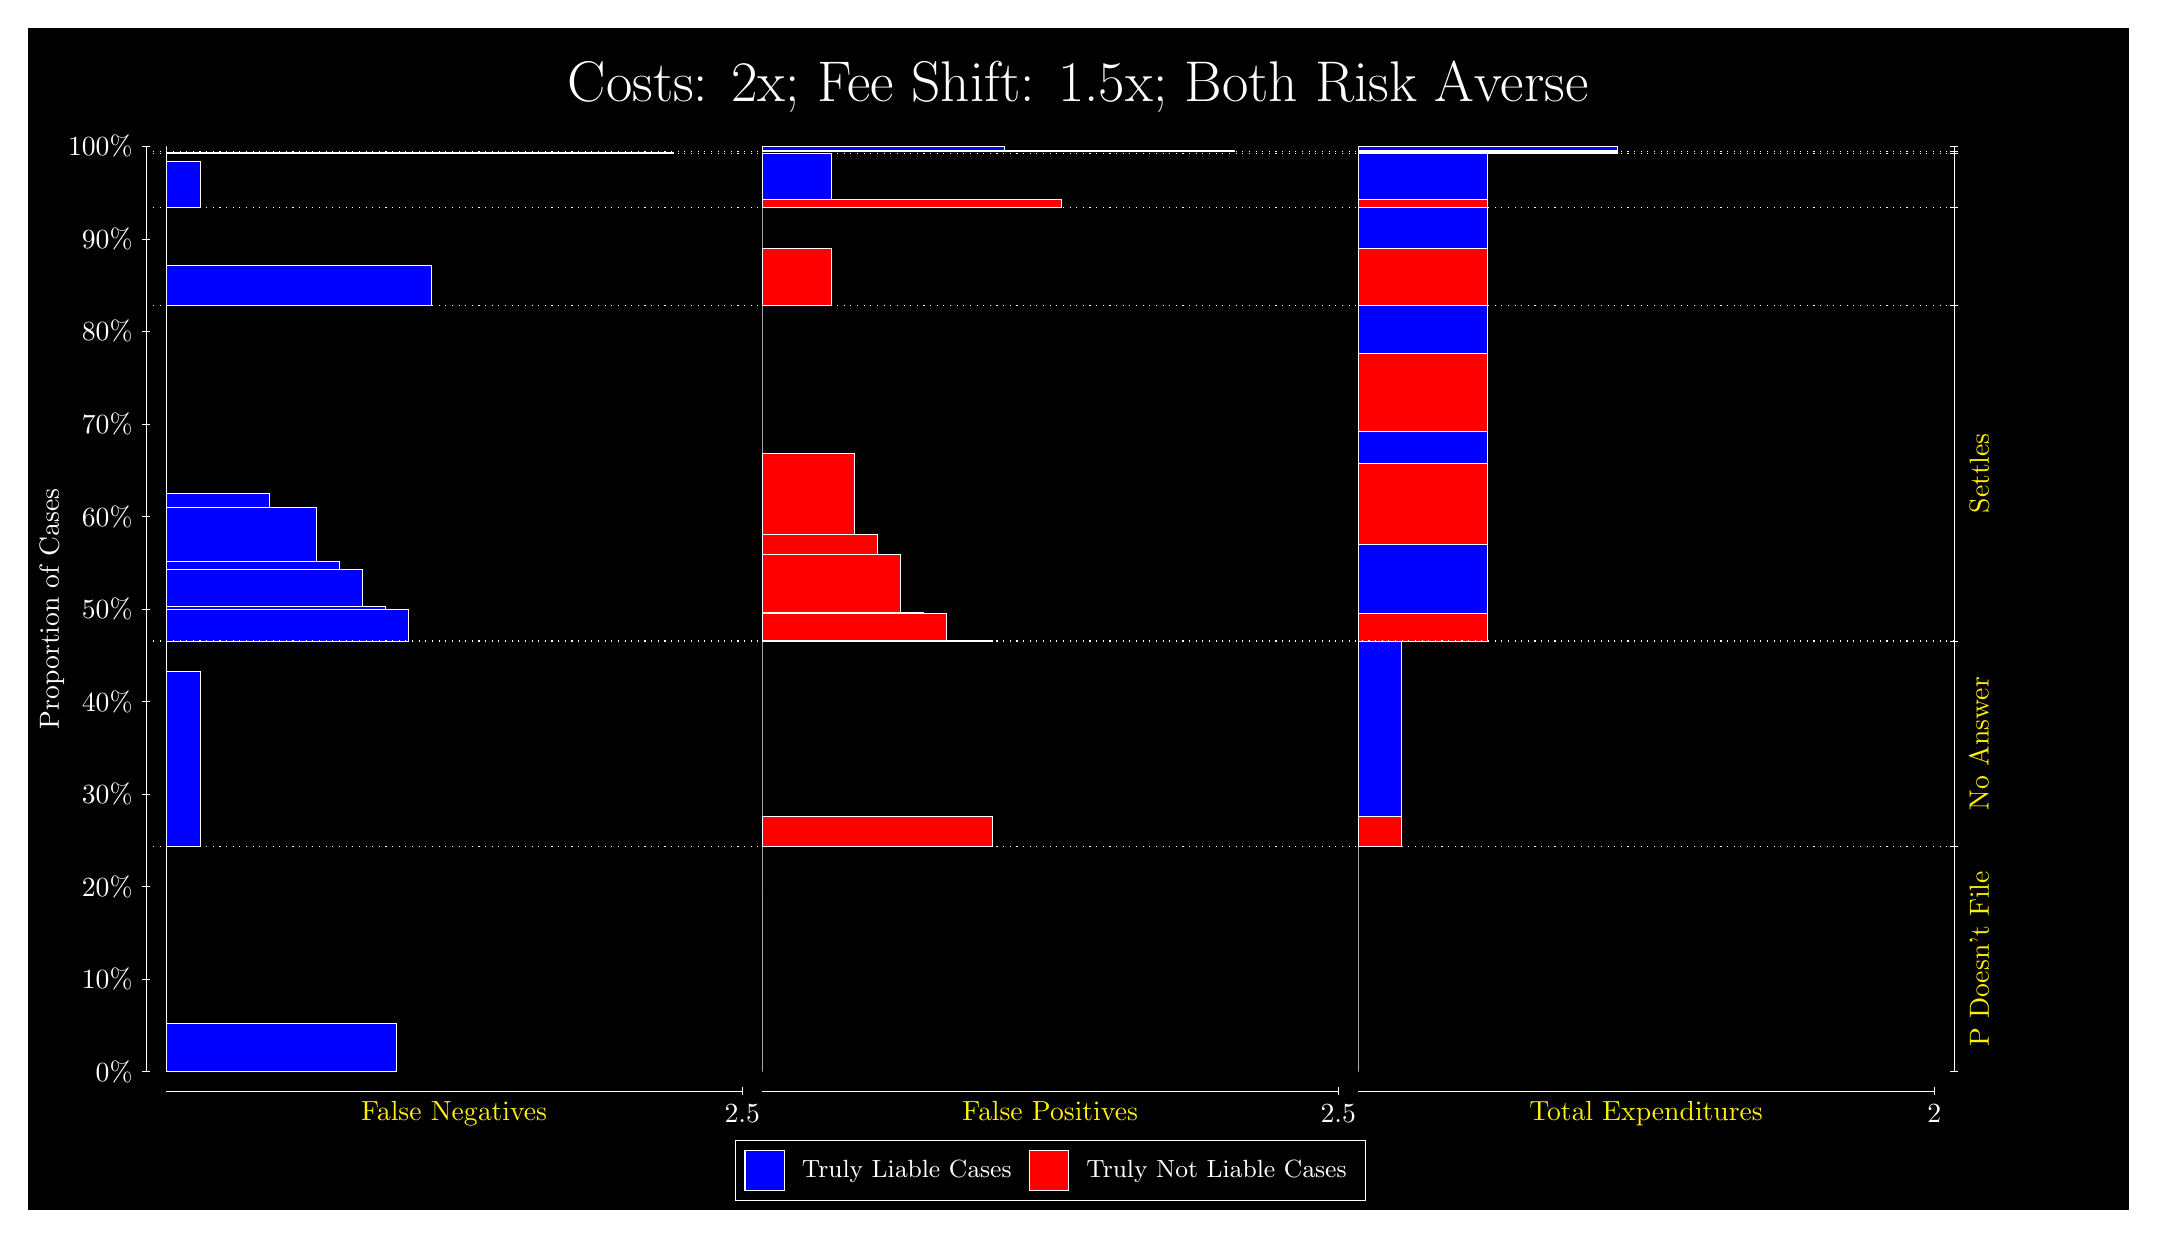
\begin{tikzpicture}
\draw[fill=black] (0,0) rectangle (26.667,15);
\draw[text=white] (0,13.5) rectangle (26.667,15) node[midway] {\huge Costs: 2x; Fee Shift: 1.5x; Both Risk Averse};
\draw[white, very thin] (1.5,1.75) -- (1.5,13.5);
\node[rotate=90, text=white, anchor=center] at (0.3, 7.625) {Proportion of Cases};
\draw[white, very thin] (1.45,1.75) -- (1.55,1.75);
\node[text=white, anchor=east] at (1.45, 1.75) {0\%};
\draw[white, very thin] (1.45,2.925) -- (1.55,2.925);
\node[text=white, anchor=east] at (1.45, 2.925) {10\%};
\draw[white, very thin] (1.45,4.1) -- (1.55,4.1);
\node[text=white, anchor=east] at (1.45, 4.1) {20\%};
\draw[white, very thin] (1.45,5.275) -- (1.55,5.275);
\node[text=white, anchor=east] at (1.45, 5.275) {30\%};
\draw[white, very thin] (1.45,6.45) -- (1.55,6.45);
\node[text=white, anchor=east] at (1.45, 6.45) {40\%};
\draw[white, very thin] (1.45,7.625) -- (1.55,7.625);
\node[text=white, anchor=east] at (1.45, 7.625) {50\%};
\draw[white, very thin] (1.45,8.8) -- (1.55,8.8);
\node[text=white, anchor=east] at (1.45, 8.8) {60\%};
\draw[white, very thin] (1.45,9.975) -- (1.55,9.975);
\node[text=white, anchor=east] at (1.45, 9.975) {70\%};
\draw[white, very thin] (1.45,11.15) -- (1.55,11.15);
\node[text=white, anchor=east] at (1.45, 11.15) {80\%};
\draw[white, very thin] (1.45,12.325) -- (1.55,12.325);
\node[text=white, anchor=east] at (1.45, 12.325) {90\%};
\draw[white, very thin] (1.45,13.5) -- (1.55,13.5);
\node[text=white, anchor=east] at (1.45, 13.5) {100\%};

\draw[white, very thin] (24.457,1.75) -- (24.457,13.5);
\draw[white, very thin] (24.407,1.75) -- (24.507,1.75);
\node[anchor=west] at (24.407, 1.75) {};
\draw[white, very thin] (24.407,4.6102) -- (24.507,4.6102);
\node[anchor=west] at (24.407, 4.6102) {};
\draw[white, very thin] (24.407,7.2181) -- (24.507,7.2181);
\node[anchor=west] at (24.407, 7.2181) {};
\draw[white, very thin] (24.407,11.479) -- (24.507,11.479);
\node[anchor=west] at (24.407, 11.479) {};
\draw[white, very thin] (24.407,12.723) -- (24.507,12.723);
\node[anchor=west] at (24.407, 12.723) {};
\draw[white, very thin] (24.407,13.408) -- (24.507,13.408);
\node[anchor=west] at (24.407, 13.408) {};
\draw[white, very thin] (24.407,13.436) -- (24.507,13.436);
\node[anchor=west] at (24.407, 13.436) {};
\draw[white, very thin] (24.407,13.5) -- (24.507,13.5);
\node[anchor=west] at (24.407, 13.5) {};

\draw[white, very thin, fill=blue] (1.75,1.75) rectangle (4.6775,2.3648);
\draw[white, very thin, fill=red] (1.75,2.3648) rectangle (1.75,4.6102);
\draw[white, very thin, fill=blue] (1.75,4.6102) rectangle (2.1891,6.8321);
\draw[white, very thin, fill=red] (1.75,6.8321) rectangle (1.75,7.2181);
\draw[white, very thin, fill=blue] (1.75,7.2181) rectangle (4.8239,7.6253);
\draw[white, very thin, fill=blue] (1.75,7.6253) rectangle (4.5312,7.66);
\draw[white, very thin, fill=blue] (1.75,7.66) rectangle (4.2384,8.1264);
\draw[white, very thin, fill=blue] (1.75,8.1264) rectangle (3.9457,8.2263);
\draw[white, very thin, fill=blue] (1.75,8.2263) rectangle (3.6529,8.9118);
\draw[white, very thin, fill=blue] (1.75,8.9118) rectangle (3.0674,9.0995);
\draw[white, very thin, fill=red] (1.75,9.0995) rectangle (1.75,11.479);
\draw[white, very thin, fill=blue] (1.75,11.479) rectangle (5.1167,11.99);
\draw[white, very thin, fill=red] (1.75,11.99) rectangle (1.75,12.723);
\draw[white, very thin, fill=blue] (1.75,12.723) rectangle (2.1891,13.304);
\draw[white, very thin, fill=red] (1.75,13.304) rectangle (1.75,13.408);
\draw[white, very thin, fill=blue] (1.75,13.408) rectangle (8.1906,13.421);
\draw[white, very thin, fill=red] (1.75,13.421) rectangle (1.75,13.436);
\draw[white, very thin, fill=red] (1.75,13.436) rectangle (1.75,13.449);
\draw[white, very thin, fill=blue] (1.75,13.449) rectangle (1.75,13.5);
\draw[white, very thin, fill=red] (9.3189,1.75) rectangle (9.3189,3.9955);
\draw[white, very thin, fill=blue] (9.3189,3.9955) rectangle (9.3189,4.6102);
\draw[white, very thin, fill=red] (9.3189,4.6102) rectangle (12.246,4.9962);
\draw[white, very thin, fill=blue] (9.3189,4.9962) rectangle (9.3189,7.2181);
\draw[white, very thin, fill=red] (9.3189,7.2181) rectangle (12.246,7.2319);
\draw[white, very thin, fill=red] (9.3189,7.2319) rectangle (11.661,7.5733);
\draw[white, very thin, fill=red] (9.3189,7.5733) rectangle (11.368,7.5841);
\draw[white, very thin, fill=red] (9.3189,7.5841) rectangle (11.075,8.3229);
\draw[white, very thin, fill=red] (9.3189,8.3229) rectangle (10.783,8.5706);
\draw[white, very thin, fill=red] (9.3189,8.5706) rectangle (10.49,9.5975);
\draw[white, very thin, fill=blue] (9.3189,9.5975) rectangle (9.3189,11.479);
\draw[white, very thin, fill=red] (9.3189,11.479) rectangle (10.197,12.211);
\draw[white, very thin, fill=blue] (9.3189,12.211) rectangle (9.3189,12.723);
\draw[white, very thin, fill=red] (9.3189,12.723) rectangle (13.125,12.827);
\draw[white, very thin, fill=blue] (9.3189,12.827) rectangle (10.197,13.408);
\draw[white, very thin, fill=red] (9.3189,13.408) rectangle (9.3189,13.423);
\draw[white, very thin, fill=blue] (9.3189,13.423) rectangle (9.3189,13.436);
\draw[white, very thin, fill=red] (9.3189,13.436) rectangle (15.32,13.449);
\draw[white, very thin, fill=blue] (9.3189,13.449) rectangle (12.393,13.5);
\draw[white, very thin, fill=red] (16.888,1.75) rectangle (16.888,3.9955);
\draw[white, very thin, fill=blue] (16.888,3.9955) rectangle (16.888,4.6102);
\draw[white, very thin, fill=red] (16.888,4.6102) rectangle (17.437,4.9962);
\draw[white, very thin, fill=blue] (16.888,4.9962) rectangle (17.437,7.2181);
\draw[white, very thin, fill=red] (16.888,7.2181) rectangle (18.534,7.5733);
\draw[white, very thin, fill=blue] (16.888,7.5733) rectangle (18.534,8.4465);
\draw[white, very thin, fill=red] (16.888,8.4465) rectangle (18.534,9.4733);
\draw[white, very thin, fill=blue] (16.888,9.4733) rectangle (18.534,9.8805);
\draw[white, very thin, fill=red] (16.888,9.8805) rectangle (18.534,10.878);
\draw[white, very thin, fill=blue] (16.888,10.878) rectangle (18.534,11.479);
\draw[white, very thin, fill=red] (16.888,11.479) rectangle (18.534,12.211);
\draw[white, very thin, fill=blue] (16.888,12.211) rectangle (18.534,12.723);
\draw[white, very thin, fill=red] (16.888,12.723) rectangle (18.534,12.827);
\draw[white, very thin, fill=blue] (16.888,12.827) rectangle (18.534,13.408);
\draw[white, very thin, fill=red] (16.888,13.408) rectangle (20.181,13.423);
\draw[white, very thin, fill=blue] (16.888,13.423) rectangle (20.181,13.436);
\draw[white, very thin, fill=red] (16.888,13.436) rectangle (20.181,13.449);
\draw[white, very thin, fill=blue] (16.888,13.449) rectangle (20.181,13.5);
\draw[white, dotted] (1.5,4.6102) -- (24.457,4.6102);
\draw[white, dotted] (1.5,7.2181) -- (24.457,7.2181);
\draw[white, dotted] (1.5,11.479) -- (24.457,11.479);
\draw[white, dotted] (1.5,12.723) -- (24.457,12.723);
\draw[white, dotted] (1.5,13.408) -- (24.457,13.408);
\draw[white, dotted] (1.5,13.436) -- (24.457,13.436);
\draw[white, very thin] (1.75,1.5) -- (9.0689,1.5);
\node[text=yellow, anchor=north] at (5.4094, 1.5) {False Negatives};
\draw[white, very thin] (9.0689,1.45) -- (9.0689,1.55);
\node[text=white, anchor=north] at (9.0689, 1.45) {2.5};

\draw[white, very thin] (9.3189,1.5) -- (16.638,1.5);
\node[text=yellow, anchor=north] at (12.978, 1.5) {False Positives};
\draw[white, very thin] (16.638,1.45) -- (16.638,1.55);
\node[text=white, anchor=north] at (16.638, 1.45) {2.5};

\draw[white, very thin] (16.888,1.5) -- (24.207,1.5);
\node[text=yellow, anchor=north] at (20.547, 1.5) {Total Expenditures};
\draw[white, very thin] (24.207,1.45) -- (24.207,1.55);
\node[text=white, anchor=north] at (24.207, 1.45) {2};

\node[text=yellow, centered, rotate=90] at (24.777, 3.1801) {P Doesn't File};
\node[text=yellow, centered, rotate=90] at (24.777, 5.9142) {No Answer};
\node[text=yellow, centered, rotate=90] at (24.777, 9.3485) {Settles};





\draw (12.978300999999998,1.5) node[draw=none] (baseCoordinate) {};
\begin{scope}[align=center]
        \matrix[scale=0.5, draw=white, below=0.5cm of baseCoordinate, nodes={draw}, column sep=0.1cm]{
            \node[rectangle, draw, minimum width=0.5cm, minimum height=0.5cm, fill=blue] {}; &
            \node[draw=none, font=\small, text=white] (B) {Truly Liable Cases}; &
            \node[rectangle, draw, minimum width=0.5cm, minimum height=0.5cm, fill=red] {}; &
            \node[draw=none, font=\small, text=white] (B) {Truly Not Liable Cases}; \\
            };
\end{scope}

\end{tikzpicture}
\end{document}